    \subsection{Central Detector}
        Overview: The Central Detector spans roughly 35 to 125 degrees, and contains 4 sub-detectors, all in a 5 Tesla solenoidal field. The 5 detectors are: SVT, MMVT, CTOF, and CND. 
        \subsubsection{SVT}
            The Silicon Vertex Tracker (SVT) covers from 35 to 125 degrees in $\theta$. Has 8 layers (4 concentric rings) with 10, 14, 18, and 24 sectors respectively, double sided. 2$\pi$ angular coverage. Read out with ASICs- FSSR2s. Designed to operate at $10^{35}$ luminosity, momentum resolution of $\sim$ 5\% for 1 GeV particles with $\theta$ = 90 degrees. 42 cm long, 4 cm wide, 0.4 cm thick. Spatial resolution of 50 $\mu$m, momentum resolution $\sim$ 5\%, theta resolution 10 mrad, phi resolution 5 mrad.  33,792 total readout channels. Sensor thickness is 320 $\mu$m, readout pitch 156 $\mu$ m.Supported by rohacell and carbon fiber backing to reduce material budget, at $\sim 1\%$ of a radiation length.
            
            \begin{figure}[H]
    			\centering
    			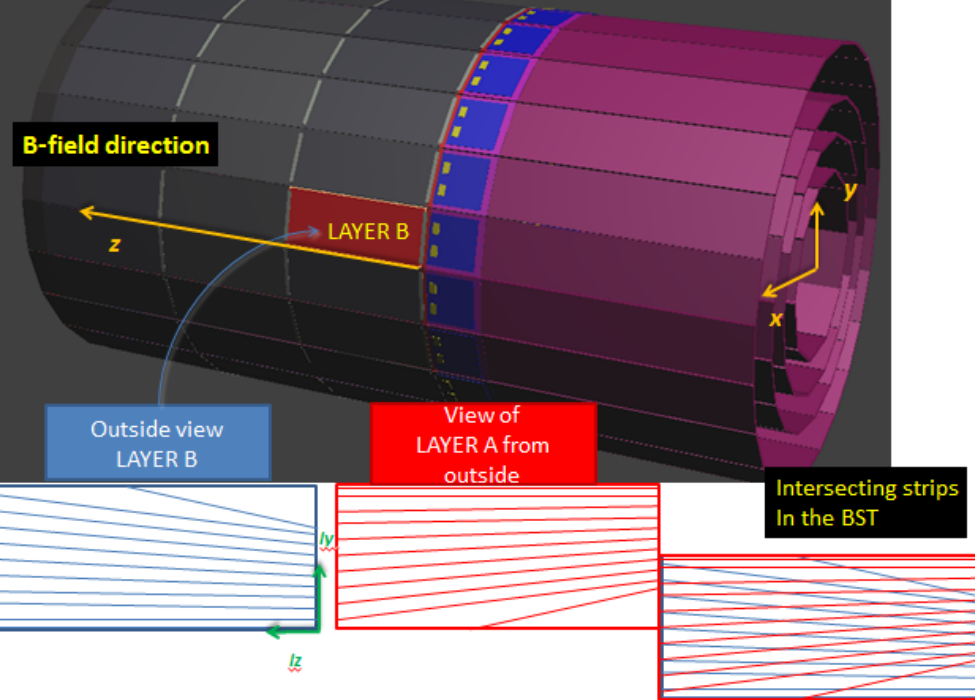
\includegraphics[width=12cm]{Chapters/Ch2-Experiment/clas-12-system/pics/cd/svt.PNG}
    			\caption{Silicon Vertex Tracker}
			\end{figure}  
			
			
			 \begin{figure}[H]
    			\centering
    			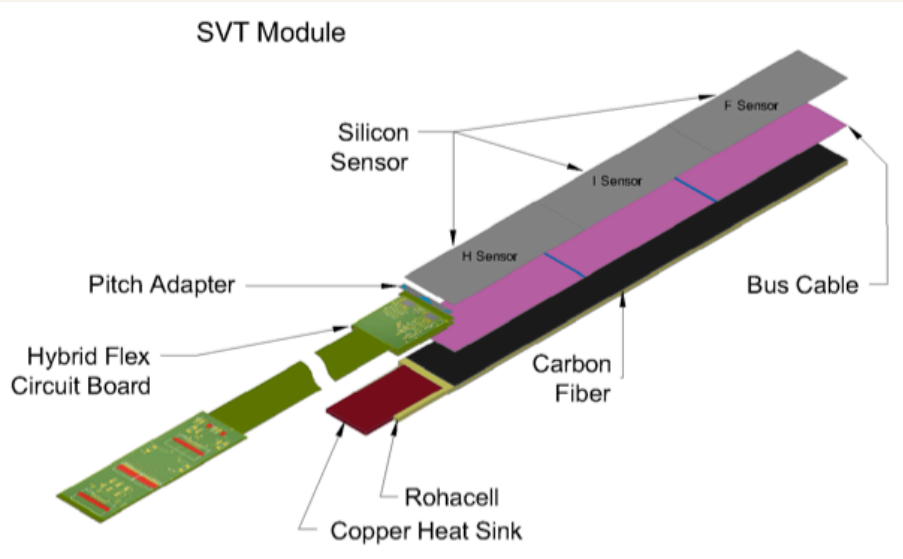
\includegraphics[width=12cm]{Chapters/Ch2-Experiment/clas-12-system/pics/cd/svt-module.PNG}
    			%\caption{SVT Strip}
			\end{figure}  
			
		
		\subsubsection{MMVT}
		    Composed of two parts: a \textbf{Barrel Tracker} and a \textbf{Forward Tracker}. PCB is 200 $\mu$m thick, 0.3\% of a radiation length. 20 MHz sampling frequency. Time resolution of 10 ns. 500 $\mu$m strip pitch.\\
		    \textbf{Advantages of MMVT for CLAS12 :} \\
		    Price: much cheaper compared to SVT. For large area, the price become rapidly prohibitive.
		    Material: Since it is a gasesous detector, it is good for the material budget.
		    Physics Requirements: Not as good spatial resolution as SVT, but can resolve polar angle better. Optimal perform ace is actually achieved with a combination of both detectors are used.
		    \newline
		    Overall momentum uncertainty ($\sigma_p$/p) = 1.6\%. $\sigma_{\theta}$ = 1.4 mrad.  $\sigma_{\phi}$ = 2.6 mrad.  $\sigma _{z}$ = 270 mm.  
		    \subsubsection{Barrel Tracker}
		        18 cylindrical detectors arranged in 6 layers. Covers 35 to 125 degrees. 15,000 readout elements.Gas Mixture 90\% Argon, 10\% isobutane. 3 mm drift gap. 5 kV/cm field. 75\% mesh transparency.
		    \subsubsection{Forward Tracker}
		        6 circular, flat detectors from 6 to 29 degrees in $\theta$. Improves vertex resolution by a factor of up to 10x compared to just the drift chambers along. 6,000 readout elements. 80\% neon, 10\% ethane, 10\% Carbon Tetrafluoride. 5 mm drift gap. 1kV/cm field. 100\% mesh transparency.
		        
		        
		        						
									
			 \begin{figure}[H]
    			\centering
    			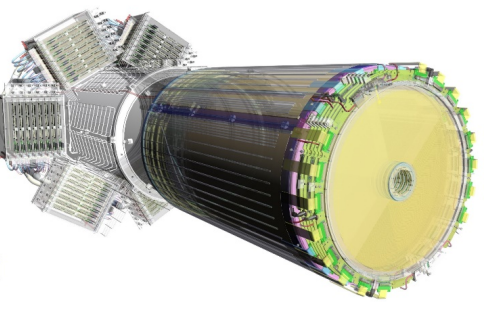
\includegraphics[width=12cm]{Chapters/Ch2-Experiment/clas-12-system/pics/cd/MVT.PNG}
    			%%\caption{SVT Strip}
			\end{figure}
 
    
        \subsubsection{CTOF}
            Central for PID purposes. Divides into 48 1 meter long plastic scintillators with double sided PMT readout.PMTs are in the 0.1 T fringe field region and enclosed in magnetic shielding. 65 picosecond timing resolution. 35 to 125 degrees, 2 $\pi$ in polar angle. 3 cm x 3 cm scintillator planks. Pion/Kaon separation up to 0.64 GeV, Kaon/proton separation up to 1 GeV, pion proton separation up to 1.25 GeV.  
            
            						
			 \begin{figure}[H]
    			\centering
    			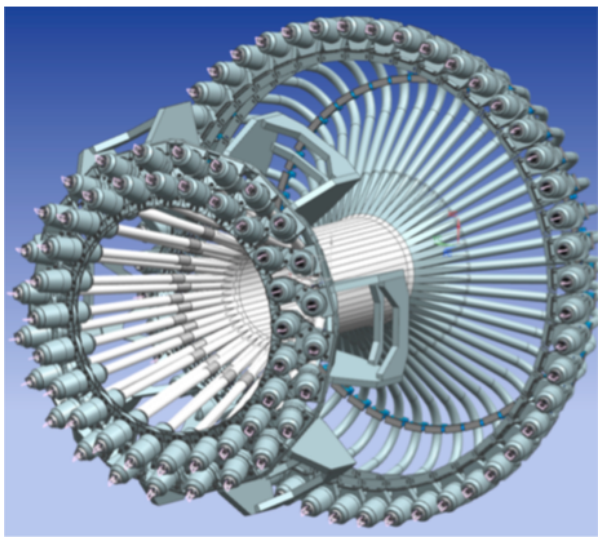
\includegraphics[width=12cm]{Chapters/Ch2-Experiment/clas-12-system/pics/cd/CTOF.PNG}
    			%%\caption{SVT Strip}
			\end{figure}
            
 
		\subsubsection{CND}
		    Detects 0.2-1 GeV neutrons. 3 layers, 48 paddles per layer. Plastic scintillator, 3 cm x 3cm, 0.7 meters  long. Neutron detection efficiency $\sim$ 10\%. 130 picosecond timing resolution, 2 degrees angular resolution (polar and azimuth).
            
            						
			 \begin{figure}[H]
    			\centering
    			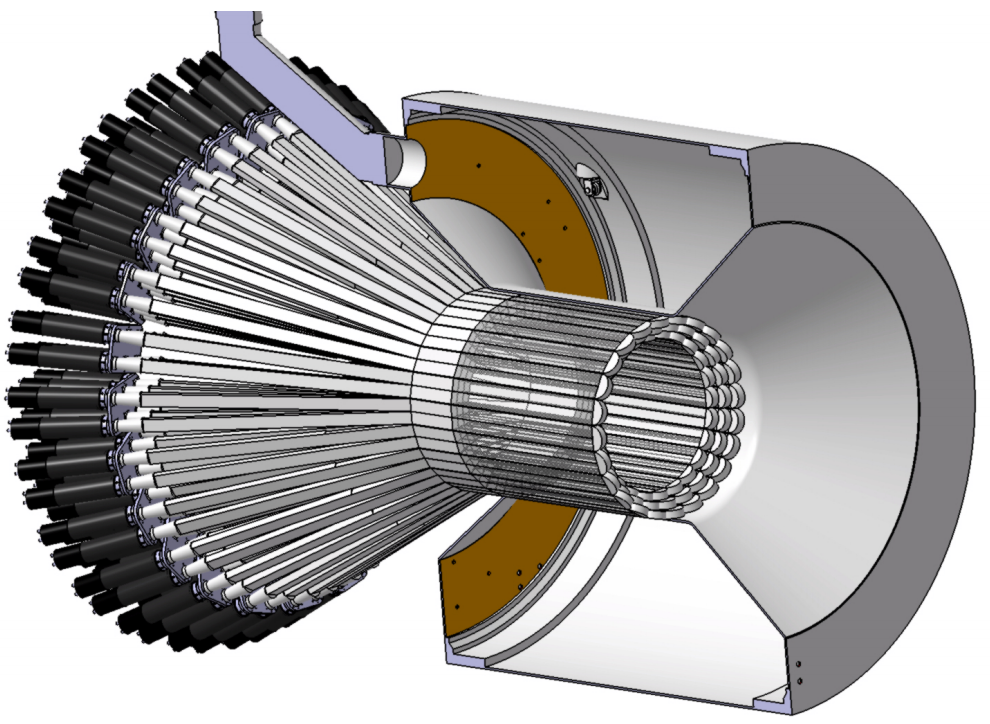
\includegraphics[width=12cm]{Chapters/Ch2-Experiment/clas-12-system/pics/cd/CND.PNG}
    			%%\caption{SVT Strip}
			\end{figure} 

		\subsubsection{Solenoid}
		    5 Tesla super conducting magnet, uniform field ($\Delta$B/B = $10^-4$). Weakest at small angles, strongest at large angles. Opening polar angle of 40 degrees. Momentum range of interest 0.3 to 1.3 GeV. 18 Megajoules stored energy. 85 cm in diameter, 4.2 Kelvin operation. 
		    
    